%% \begin{table*}[t]
%%     \centering
%%     \begin{tabular}{p{17em}p{14em}p{14em}}
%%         \toprule
%%     \textbf{Assumption or Feature}                          & \textbf{Associated Implementation}  & \textbf{Prevalence}    \\
%%     \midrule
%%     Domain will use actionable DMARC policies   & DMARC none & Two thirdsSecurity of popular Alexa domains that have DMARC \\
%%     %\hline
%%     Each domain uses its own infrastructure  & Shared SPF record    & All providers \alex{Fastmail? Forwarding infra?}  \\
%%     Quarantining an email neutralizes its threat    & Quarantine instead of reject    & Outlook, Fastmail, GMX and Inbox.lv \\
%%     Allowing users to override DMARC decisions    & Domain whitelisting    & All providers  \\
%%     %\hline

%%     Users only forward to accounts they control   & Open forwarding    & Outlook, Fastmail and Mail2world.com \\
%%     Forwarded email from large providers are likely benign  & Relaxed validation & Gmail, Outlook and Mail.ru   \\
%%     %    & Overtrust other providers    & Gmail    \\
%%     %    & ARC bug    & Zoho    \\
%%     %    & UI bug & Gmail \\
%%     Every email is legitimate & Not enforcing DMARC & Gaggle.email and Mail2world.com\\
%%     \bottomrule
%%     \end{tabular}
%%     \captionof{table}{Summary of vulnerable designs and assumptions that attackers can exploit with forwarding.}
%%     \label{tab:assumptions_and_prevalence}
%%     \end{table*}

\begin{table*}[t]
    \centering
    \small
%    \begin{tabular}{lp{17em}p{14em}p{14em}}
    \begin{tabular}{p{0.08\textwidth}p{0.32\textwidth}p{0.3\textwidth}p{0.18\textwidth}}
        \toprule
&     \textbf{Security Assumption or Feature} & \textbf{Implementation Aspect}  & \textbf{Prevalence}    \\
    \midrule
    \S~\ref{subsubsec:dmarc_none} &    Domain will use actionable DMARC policies   & DMARC None & Two-thirds of Alexa Top 1M\\
% Two-thirds of popular Alexa domains using DMARC
    %\hline
    \S~\ref{subsubsec:spf_incorporation} &  Each domain uses its own infrastructure  & Shared SPF record    & All providers \\
    \S~\ref{subsubsec:quarantine_instead_of_reject}    & Quarantining is sufficient    & Quarantine instead of reject    & Outlook, Fastmail, GMX, Inbox.lv, Pobox \\
    \S~\ref{subsubsec:whitelist}    & Per-user DMARC overrides are fate-sharing    & Domain whitelisting    & All providers  \\ [0.15in]
    %\hline

    \S~\ref{subsubsec:open_forwarding}    & Users only forward to accounts they control   & Open forwarding    & Ten providers including Outlook and Fastmail\\
    \S~\ref{subsubsec:relaxed_validation}    & Forwarded email from large providers benign  & Relaxed validation & Gmail, Outlook, Mail.ru   \\
    \S~\ref{subsubsec:unsolicited_dkim}    & Adding DKIM signature increases deliverability & Unsolicited DKIM signatures & iCloud, Runbox,  Hushmail\\


    %    & Overtrust other providers    & Gmail    \\
    %    & ARC bug    & Zoho    \\
    %    & UI bug & Gmail \\
%    & Every email is legitimate & Not enforcing DMARC & Gaggle.email and Mail2world.com\\
    \bottomrule
    \end{tabular}
    \captionof{table}{Summary of vulnerable security assumptions and forwarding features, the aspect of their implementation that leads to the vulnerability, and the prevalence of the vulnerability.
    }
    \label{tab:assumptions_and_prevalence}
%    \vspace*{-0.2in}
    \end{table*}

% \section{Assumptions Violations and Implementation Errors in Practice}
% \section{Vulnerable Security Assumptions and Forwarding Mechanisms}
% \section{Vulnerabilities, Assumptions and Bugs}
\section{Assumptions and Vulnerable Features}
\label{sec:assumptions}

In this section, we describe a range of email design and
implementation weaknesses that lead to forwarding vulnerabilities.
We start by exploring four assumptions made by anti-spoofing mechanisms
that email forwarding can bypass and violate.  We then examine
three vulnerable forwarding features in the major forwarding
approaches.

%Finally, we also identify
%three
%implementation
%vulnerabilities that are less fundamental, but can still lead to email
%spoofing via forwarding.
In each of these cases, we use active
measurements --- either of mail services themselves or the DMARC policies
as stored in DNS --- to document the prevalence of each issue
among prominent domains and
providers (summarized in Table~\ref{tab:assumptions_and_prevalence}).
In the remainder of this section, we discuss the measurement
methodology used to investigate and identify these issues and
describe each vulnerability in turn.  In the next section,
% (Section~\ref{sec:attacks})
we then show how these vulnerabilities can
be combined to create complete and effective spoofing attacks
involving a broad array of popular and sensitive domains.

% header rewriting performed during forwarding and vulnerabilities across these two categories to launch attacks that can successfully spoof email from thousands of prominent domains, such \dns{state.gov} and \dns{hulu.com}.

% Additionally, we discuss three implementation vulnerabilities that enable a few novel attacks in Section~\ref{sec:attacks}, which we uncovered during the course of our experiments.



% In this section we examine a set of vulnerable assumptions and implementations across popular email providers and anti-spoofing mechanisms,
% and preview how an attacker can use email forwarding to violate and exploit these design decisions.
% Table~\ref{tab:assumptions_and_prevalence} summarizes our findings, as well as the prevalence of each vulnerability across the email ecosystem.

\subsection{Methodology}
\label{sec:methodology}

%% \geoff{how much of this part of the methodology overlaps with
%%   the methodology described in III.B?
%%   if it is the same, then we can just refer back to III.B}\alex{III.B is rather simple. This seems to be a more detailed version of what's in III.B}
%%   \grant{The first sentence above has some repetition, but I think the rest might be distinct?}\alex{note from the discussion Geoff and I had: We don't run seperate experiments for section 3 and 4, so it might be less confusing if we describe everything here and forward reference in sec 3. Also todo@Geoff, revisit our experiments details and see if anything needs to be added back}

For our experiments we created test \textit{forwarding} accounts on all 20 forwarding services,
test \textit{recipient} accounts on all 16 major
email providers, and mail servers for domains we control as
the \textit{sending} accounts.
%
%% For the email providers, we created test accounts on each platform and
%% configured them to forward email to accounts we controlled.
%% We created mailing lists using each of the services and performed a
%% similar analysis that collected the headers of email we sent to each
%% list.
%
For Google Groups and Gaggle, we created mailing lists under our
university's existing service and at \dns{gaggle.email}, respectively.
The other two mailing list services (Listserv and Mailman) rely upon a
third-party backend mail server; we used
Postfix~\cite{ThePostf34:online} as the backend with DMARC
enforced. We then created mailing lists under new domains we acquired
for testing (\eg, \dns{list@listserv.ourdomain.com}).

%% We recorded the resulting headers at both the forwarder and the final
%% recipients for analysis.

For each combination of forwarding and recipient accounts, we sent
email using three different control domains in the FROM headers, each
with the same SPF configuration but with distinct DMARC policies:
\textsc{None}, \textsc{Quarantine}, and \textsc{Reject}.
%
Some services (\eg, Gmail and Outlook) will mark email messages sent
from new domains as spam until there is sufficient user interaction
with those messages.  To avoid this startup effect, we ``warmed up''
our domains using a series of legitimate exchanges.  In particular,
from each domain, we sent legitimate (\ie, unspoofed) email that
passed SPF, DKIM and DMARC to our accounts at each provider.  Any
message that was delivered to the spam folder we manually marked as
``not spam''.  After this warm up period, we validated that legitimate
(\ie, unspoofed) email from our domains was properly delivered to
account inboxes in all cases.
% for all email providers.

Having primed our accounts, we assessed the prevalence of each vulnerability by
% ran a series of experiments that
sending legitimate and spoofed email messages to all
pairwise combinations of our forwarding and recipient accounts.\footnote{Our code for automatically sending these messages is available upon request.}  We
analyzed the headers and outcomes of these attempts, and recorded
which parties exhibited vulnerable behavior.  In particular, we
configured all forwarders to forward email messages to all receivers
and recorded whether each message was delivered to the inbox, spam
folder, or rejected without delivery by each receiver.  We also noted
whether any UI warning was shown in the native web-based MUA. 


% email ecosystem.


%% \geoff{did we also do
%%   some warm up to establish baseline benign conversations?}\alex{we
%%   did, but I think we removed that part intentionally to avoid any
%%   confusion. We can add them back}

% We start with a set of three new domains under our control.  We
% configure all three with the same SPF configuration, while each of the
% individual domains have a DMARC policy none, quarantine, and reject,
% respectively.  We use these domains in the FROM headers in all of our
% email messages, so that our measurements do not affect users of any
% other domains.

% We then ``warm up'' our domains so that they are treated like any
% other domains by the providers. This ``warm up'' phase is necessary as some providers (e.g., Gmail) would quarantine email messages from a domain if it has never seen an email from that domain before. We ``warm up'' our domain by sending legitimate email messages
% from these domains that pass SPF, DKIM and DMARC to accounts under our
% control at each email provider.  We also manually mark our email
% messages as ``not spam'' if they are delivered to the spam folder in
% the warm-up stage.  After the warm-up stage, legitimate email messages
% from our domains are properly delivered to account inboxes for all email providers.

% We then send legitimate and spoofed email messages from our domains to
% forwarding accounts and record whether a message is forwarded by
% default.  We consider all nine providers and four mailing lists as
% forwarders.  We send spoofed email messages from a server we own that
% is not allowed in the SPF records of our domains.

% We study each receiver's behavior for both legitimate and spoofed
% forwarded email messages. We only consider the nine mail providers as
% receivers, as mailing lists are rarely the destination of email. We
% configure all forwarders to forward email messages to all receivers
% and record whether each message is delivered to the inbox, spam
% folder, or rejected without delivery by each receiver. We also note
% whether any UI warning indicator is displayed in the native web-based
% MUA.

% We force the forwarding of a spoofed email by manually whitelisting it
% at the forwarder. Whitelisting spoofed email messages could be done at
% most forwarders with a few exceptions. We are not able to whitelist
% spoofed email messages at Yahoo in cases where the spoofed FROM domain
% has DMARC policies quarantine or reject. Additionally, we cannot
% whitelist spoofed email messages at Google, Mail.ru and Zoho when the spoofed FROM domain has DMARC policy reject.

% We ensure that our measurement results are reliable by repeating the
% above process with another set of three domains and fresh email
% accounts. We are also aware that all mail providers we study have
% implemented anti-spam systems, which could interfere with our
% measurement results. To minimize the interference from those systems,
% we only send email messages with legitimate content. In cases where we
% observe an inconsistency in a provider's behavior between multiple
% trials (potentially due to triggering the anti-spam system), we
% perform additional measurements with fresh accounts.



% Subsequently, in Section~\ref{sec:attacks}, we show how attackers can combine
% email forwarding with several vulnerabilities to launch successful attacks, allowing them to reliably spoof email from thousands of prominent domains, such \dns{state.gov} and \dns{hulu.com}.
% that email providers and security mechanisms make and
% how forwarding allows an attacker to violate each assumption.
% Additionally, for each vulnerability, we measured and report which email services are impacted.
% In Section~\ref{subsec:assumptions}, we examine a list of assumptions and why they can cause security concerns. Further, to understand whether these security concerns are real, we perform controlled experiments that allow us to observe implementation decisions made by each party that are related to these assumptions.

%%%%%%%%%%%%%%%%%%%%%%%%%%%%%%%%%%%%%%%%%%%%%%%%%%%%%%%%%%%%%%%%%%%%%%%%%

% We start by sending legitimate and spoofed email messages from domains we control to all forwarders. We consider all nine providers and four mailing list services as forwarders. Next, we try forwarding email messages from all forwarders to all receivers. We only consider the nine mail providers as receivers, as mailing lists are rarely the destination of an email. We note and record implementation decisions made by each party that are related to the assumptions we listed.
%
% We ensure that our measurement results are reliable by doing the above measurement twice with two distinct sets of domains that we control. We are also aware that all mail providers we study have
% implemented anti-spam systems, which could interfere with our
% measurement results. To minimize the interference from those systems,
% we only send email messages with legitimate content. In cases where we
% observe an inconsistency in a provider's behavior between multiple trials (potentially due to triggering the anti-spam system), we perform additional measurements with fresh accounts.


% Table~\ref{tab:assumptions_and_prevalence} lists our results. \alex{I should elaborate?}. In the process of doing our measurement, we further observe two implementation errors made by Gmail and Zoho, which we detail in Section~\ref{subsec:implementation_errors}.

%%%%%%%%%%%%%%%%%%%%%%%%%%%%%%%%%%%%%%%%%%%%%%%%%%%%%%%%%%%%%%%%%%%%%%%%%

% We start with a set of three new domains under our control.  We
% configure all three with the same SPF configuration, while each of the
% individual domains have a DMARC policy none, quarantine, and reject,
% respectively.  We use these domains in the FROM headers in all of our
% email messages, so that our measurements do not affect users of any
% other domains.

% We then ``warm up'' our domains so that they are treated like any
% other domains by the providers. This ``warm up'' phase is necessary as some providers (e.g., Gmail) would quarantine email messages from a domain if it has never seen an email from that domain before. We ``warm up'' our domain by sending legitimate email messages
% from these domains that pass SPF, DKIM and DMARC to accounts under our
% control at each email provider.  We also manually mark our email
% messages as ``not spam'' if they are delivered to the spam folder in
% the warm-up stage.  After the warm-up stage, legitimate email messages
% from our domains are properly delivered to account inboxes for all email providers.

% We then send legitimate and spoofed email messages from our domains to
% forwarding accounts and record whether a message is forwarded by
% default.  We consider all nine providers and four mailing lists as
% forwarders.  We send spoofed email messages from a server we own that
% is not allowed in the SPF records of our domains.

% We study each receiver's behavior for both legitimate and spoofed
% forwarded email messages. We only consider the nine mail providers as
% receivers, as mailing lists are rarely the destination of email. We
% configure all forwarders to forward email messages to all receivers
% and record whether each message is delivered to the inbox, spam
% folder, or rejected without delivery by each receiver. We also note
% whether any UI warning indicator is displayed in the native web-based
% MUA.

% We force the forwarding of a spoofed email by manually whitelisting it

% at the forwarder. Whitelisting spoofed email messages could be done at
% most forwarders with a few exceptions. We are not able to whitelist
% spoofed email messages at Yahoo in cases where the spoofed FROM domain
% has DMARC policies quarantine or reject. Additionally, we cannot
% whitelist spoofed email messages at Google, Mail.ru and Zoho when the spoofed FROM domain has DMARC policy reject.

% We ensure that our measurement results are reliable by repeating the
% above process with another set of three domains and fresh email
% accounts. We are also aware that all mail providers we study have
% implemented anti-spam systems, which could interfere with our
% measurement results. To minimize the interference from those systems,
% we only send email messages with legitimate content. In cases where we
% observe an inconsistency in a provider's behavior between multiple
% trials (potentially due to triggering the anti-spam system), we
% perform additional measurements with fresh accounts.




% For assumptions made by senders, we use results reported in prior work~\cite{tatang2021evolution}. For assumptions made by forwarders and receivers, we perform our own measurements as detailed in Section~\ref{subsec:measure_assumptions}.


% \subsection{Assumptions Made in Practice}
\subsection{Email Security Assumptions}
\label{subsec:assumptions}
Anti-spoofing mechanisms define a set of validation procedures which
both explicitly and implicitly rely on assumptions about the behavior
of domain holders, email providers and users.  Here we identify four
such assumptions that are crucial to these defenses in the direct
single-hop delivery context, but do not necessarily hold in the
presence of email forwarding.

% communication,


% In this subsection, we explore different design decisions and assumptions made by email protocols and providers, why forwarding makes them vulnerable to attacks, real-world implementations associated with each vulnerable design.
% Here, we focus on vulnerabilities that are difficult to fix without altering standard email practices or requiring additional action from users and organizations.
% cover harder-to-fix assumptions, why they can be problematic, and real-world implementations associated with each assumption.

\subsubsection{Domains use actionable DMARC policies}
\label{subsubsec:dmarc_none}
DMARC enables recipients to authenticate whether an email truly
originates from its purported sending domain.  However, when a
recipient encounters a spoofed or illegitimate email that fails
authentication, DMARC relies on the true domain owner to specify a
policy for how to treat such email.  This design assumes that domain
owners will use DMARC policies that result in protective
actions, such as \textsc{Quarantine} or \textsc{Reject}.  When a
domain owner chooses a weaker policy, mail providers deliver the
illegitimate email to a user's inbox even if the DMARC authentication
fails, in accordance with email standards (RFC 7489~\cite{rfc7489}).
Unfortunately, prior work has shown that a large number of domains use
weak DMARC policies of
\textsc{None}~\cite{hu_end--end_nodate,tatang2021evolution,hutowardsunderstanding,
  secplaintxt, maroofi2020defensive, adoptionofschemes}, with roughly
two-thirds of the Alexa Top 1M domains employing such a policy (as of
May 2020).  While poor security hygiene accounts for some of this
outcome, many domains choose a weak DMARC enforcement policy for
deliverability concerns due to incompatibility with forwarding~\cite{hutowardsunderstanding}.

% DMARC allows domain owners to specify how to authenticate emails purporting to come from their domain and to instruct mail providers on how to treat illegitimate and spoofed emails. This implicitly assumes that domains will employ good security practices by setting their DMARC policy to quarantine or reject.  Unfortunately, this policy often leaves recipients vulnerable to spoofing attacks in practice, since most providers deliver email to a user's inbox even if it fails DMARC's authentication checks;
% indeed, this behavior matches the expected behavior defined in RFC 7489~\cite{rfc7489}. While some of the domains certainly have bad security hygienes, others do this for deliverability concerns~\cite{hutowardsunderstanding}.
%
% \alex{We did not measure the number of domains w/ DMARC none ourself.}
% Unfortunately, prior work~\cite{hu_end--end_nodate,tatang2021evolution} has shown that a large number of domains use weak DMARC policies of \textsc{None}. For example, according to Tatang et al.~\cite{tatang2021evolution}, among the Alexa top domains that have DMARC configured, roughly two thirds of them have DMARC policy none (as of May 2020).

% DMARC none is no new face to the security community, and there exists a large body of literature around it~\cite{hu_end--end_nodate, hutowardsunderstanding,
% secplaintxt, maroofi2020defensive, adoptionofschemes}.
Cognizant of this reality, several major email providers have decided to take two types of security actions against email that fails DMARC authentication, regardless of the domain owner's specified policy.
First, as noted in prior work~\cite{hu_end--end_nodate} and confirmed in our own experiments, Outlook quarantines email if it fails DMARC authentication, even when the email's \textsc{FROM} domain has a weak DMARC policy of \textsc{None}.
Second, although Gmail, Onet, and Zoho deliver email that fails DMARC authentication to user inboxes, they will display a UI warning to users who read such messages.

These defenses provide protection against attackers who directly send spoofed email to their victims.  However, as we will show,
%~\ref{subsec:attack_relaxed_forwarding_validation} and~\ref{subsec:attack_none_mailing_list},
email forwarding introduces new complexity that enables attackers to bypass these ad hoc defenses, and thus leverage weak DMARC policies to successfully spoofed email from prominent domains.

% In our experiments we observed two defenses that limit the scope of
% this vulnerability for particular providers. First, as also noted by Hu \etal~\cite{hu_end--end_nodate}, if an email message is
% directly sent to Outlook from our server, Outlook always quarantines it if it fails DMARC,
% regardless of the DMARC policy of the \textsc{FROM} domain. Second, as with other providers Gmail
% and Zoho deliver such email messages to the inbox, but also displaying a UI
% warning to users when they read the message. However, as we detail later in Section~\ref{subsubsec:ui_bug}, deferring this to another component (in this case UI) implicitly assumes the UI warning component functions properly, which is not true for Gmail.
%
%
% Sadly, as we detail later, the protection mechanisms mentioned above do not apply to certain forwarded email messages, allowing an
% adversary to bypass them and deliver spoofed messages
% (Section~\ref{subsec:attack_relaxed_forwarding_validation}). We also demonstrate that when combined with certain forwarding mechanism, an adversary can launder their spoofed email messages from domains with DMARC none through mailing lists such that they look no different than legitimate ones after being forwarded (Section~\ref{subsec:attack_none_mailing_list}).


\subsubsection{Each domain uses its own infrastructure}
\label{subsubsec:spf_incorporation}
The SPF protocol predates the emergence of large third-party email providers.
As a result, SPF implicitly assumes that each organization (domain) maintains its own mailing infrastructure: that the set of authentic server IP addresses specified by a domain's SPF record is not also used by other domains or external users to send email.
Unfortunately, as documented by Liu \etal~\cite{liu2021s} and Holzbauer \etal~\cite{holzbauer2022not}, this assumption is invalid today as many organizations outsource their email infrastructure to the \emph{same} third-party providers such as Outlook and Gmail.  Hence, all of these domains have delegated the right to send on their behalf to the same third-party --- trusting that they will ensure isolation in spite of this blanket authorization.
%These large providers often share the same email infrastructure across all cust%omers (both business and personal accounts), violating the assumptions made by %SPF.

% Back when SPF was first proposed, third-party providers were not common. SPF assumes each domain maintains its own infrastructure. However, the rise of third-party providers has challenged this assumption. As documented by Liu et al~\cite{liu2021s}, third-party providers now play a dominant role in mail service provisioning. Instead having dedicated infrastructure for each customer, these third-party providers often share the same infrastructure across all customers, business or personal. However, this implementation breaks the assumption made by SPF and introduces the potential issue of email spoofing --- an adversary, who controls a personal account with the provider, can spoof as others who share the same infrastructure.

Concretely, our measurements show that all 16 email providers in our study appear to configure their email infrastructure in this shared fashion.
%\alex{VERIFY THIS IS TRUE. how do we even measure this?} \geoff{I added hedge wording}.
Additionally, at least for email messages forwarded in our experiments, all providers but one (Fastmail) use the same set of servers to send both direct email and forwarded email.
%~\alex{VERIFY}.  \geoff{we can say that it is true to the extent of the messages we sent...do any providers happen to mention this in their SPF instructions?}\alex{Updated the text a bit. I don't recall seeing any provider mentioning IPs used for forwarding.}

Since SPF no longer provides isolation in this model, the email
providers in our study effectively \emph{simulate} it by preventing users
from setting arbitrary values in their \textsc{FROM} header.  Thus,
even though each mail provider is empowered to send any email on
behalf of all their mail customers, they prevent customers from taking
advantage of this situation by \emph{internally} restricting the \textsc{FROM} headers of outbound email messages coming from a customer's domain.
%a given domain which mitigates the ability for an attacker to use
%these platforms to directly send spoofed email.
% to users.
While this defense is effective in the absence of forwarding, we will
show how open forwarding mechanisms bypass this filtering (by generating spoofed \textsc{FROM} headers from an \emph{external} server controlled by the adversary),
exposing the latent conflict between SPF's design and modern mail service
use---ultimately allowing unrestricted email spoofing.

%Unfortunately, as we show later in Section~\ref{subsec:attack_open_forwarding},
%attackers can overcome these mitigations by employing forwarding to conduct successful spoofing attacks.


\subsubsection{Quarantining is sufficient}
\label{subsubsec:quarantine_instead_of_reject}
RFC 7489~\cite{rfc5231} suggests that if an email message falls under the scope of a DMARC reject policy, then the receiving server should reject and drop it entirely. However, some providers deviate from this advice by marking it as spam and delivering it to a spam folder, assuming that quarantining a malicious email neutralizes its threat.
Our experiments found that five email providers (Outlook, Fastmail, GMX, Inbox.lv and Pobox) adopt this approach.
% believe that quarantining an email neutralizes its threat and still deliver these messages while labeling them as spam.
Figure~\ref{fig:example_ms_not_rejecting} displays an email message from our tests that shows this behavior: it fails DMARC validation, comes from a domain (\dns{state.gov}) that has a DMARC policy of \textsc{Reject}, but is nonetheless delivered
as ``spam''.

\begin{figure}[t]
    \centering
{
    \setlength{\fboxsep}{0pt}
    \setlength{\fboxrule}{0.5pt}
    \fbox{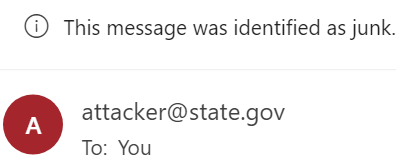
\includegraphics[clip,width=0.98\columnwidth]{fig/ss_outlook_not_rejecting.png}}
}
    %\caption{Example message that has a spoofed FROM header using a domain with DMARC policy reject.  It is delivered to an Outlook user's spam folder instead of being rejected.}
    \caption{Example message with a FROM header spoofing a domain with DMARC policy \textsc{Reject}.  Outlook delivers it to the spam folder instead of rejecting it.
    }
    \label{fig:example_ms_not_rejecting}
    \end{figure}

%
% In our experiments, we find that four email providers (Outlook, Fastmail, GMX and Inbox.lv) follow this quarantine-over-reject approach.

Because these providers quarantine the spoofed email as spam, this
design does not appear particularly dangerous.\footnote{Some in the
  mail security industry criticize this weakening of DMARC
  rules and document attacks that ``rescue'' such email from the spam folder via social engineering~\cite{Microsof7:online,Spearphi83:online}.} However, as we
will show, in combination with email forwarding and another
vulnerable feature (per-user domain whitelists in Section~\ref{subsubsec:whitelist}), attackers can override this
protection and exploit the quarantine-over-reject implementation to spoof
email from thousands of popular domains despite their strict
DMARC \textsc{Reject} policy.

%In our work, we present new attacks that show how forwarding introduces a new avenue for exploiting this design.
%In particular, when combined with other vulnerable assumptions (e.g., Section~\ref{subsubsec:whitelist}), attackers can use forwarding accounts to override these quarantine protections and exploit the header rewriting changes in different forwarding approaches to spoof email messages from thousands of popular domains.
%Because of this quarantine-over-reject policy, these attacks are successful even when the spoofed domains have a strict DMARC policy of \textsc{Reject}.

% , and the resulting emails pass both SPF and DMARC validation at the recipient's mail server.

% there have been attacks that explotied this implementation decision as reported in prior blog posts~\cite{Microsof7:online,Spearphi83:online}.
%
% Even worse, as we detail below in Section~\ref{subsubsec:whitelist}, the quarantine decision can be overridden by a malicious user and thus creates a new threat to the downstream providers, potentially allowing an adversary to forward spoofed email messages even if the spoofed FROM domain has DMARC policy reject, endangering downstream providers. Indeed,
% we show in Section~\ref{subsec:attack_open_forwarding} that when an adversary combines such policies with email forwarding and other issues described in this section, they can often spoof email messages from a wide range of domains (even if these domains have DMARC policy reject) that correctly pass both SPF and DMARC validation at the recipient's mail server.

\subsubsection{Per-user DMARC overrides are fate-sharing}
\label{subsubsec:whitelist}
Many email providers allow users to override DMARC decisions: users can whitelist domains, and as a result they will still deliver or forward email even if it fails DMARC.
% \geoff{by ``upon a user's request'', do we just mean that users can whitelist domains to override DMARC?}\alex{yes, updated the text.}
Providers offer this flexibility because it can help mitigate
errors and improve mail deliverability for the users who need it.
However, this feature implicitly assumes that this approach is
fate-sharing --- that when a user overrides DMARC decisions, the risks
of that choice are localized to the individual user account.  While
true in the single-hop context, forwarding again undermines this
assumption.  If adversaries can override DMARC decisions on a
forwarding account they control, they can use that capability to
launder spoofed mail and successfully deliver it downstream.

 % While this can be convenient in certain use cases (e.g., to increase deliverability), it also allows an adversary to potentially forward spoofed email messages. When combined with \emph{open forwarding}, whitelisting enables an adversary to forward spoofed email messages to arbitrary destination, hurting the users of downstream providers and also invalidating the assumption that quarantining an email neutralizes the threat (Section~\ref{subsubsec:quarantine_instead_of_reject}) by introducing a new threat to downstream providers.

Based on our measurements, all mail providers support this functionality in some form.
Of particular note, four of the five providers 
mentioned in Section~\ref{subsubsec:quarantine_instead_of_reject}
(Fastmail, GMX, Inbox.lv, and Pobox)
allow users to override any DMARC decision for any domains.
The fifth (Outlook) allows users to override DMARC decisions for most domains, except for a small set of frequently-spoofed domains that have DMARC policy reject (e.g., \dns{aa.com}) where Outlook appears to apply additional, special protection mechanisms.

% We do not try to whitelist spoofed email messages at mailing list services as generally an adversary cannot have access to a mailing list's configuration. Mail2World.com does not enforce DMARC, so there is no need to override the decision. For the four providers mentioned in Section~\ref{subsubsec:quarantine_instead_of_reject} that do not reject any email, we can override DMARC decisions for all domains for three of them (Fastmail, GMX and Inbox.lv). We are able to override DMARC decision for most domains for Outlook, except for a small set of frequently-spoofed domains that have DMARC policy reject (e.g., \dns{aa.com}). We suspect Outlook has special protection mechanism for these domains.
For Gmail, Hushmail, iCloud, Mail.ru, Onet, and Zoho, users can override DMARC decisions for domains with DMARC policy \textsc{None} or \textsc{Quarantine}, but not \textsc{Reject}.  Finally, for Yahoo, we can only override DMARC decisions for domains with a policy of \textsc{None}.

% but place them in the spam folder instead of the inbox

 % should be rejected but instead delivered to spam.
% The spoofed FROM domain in this case is microsoft.com, which has DMARC policy reject.

% While this vulnerability does not seem to create huge security concerns, there has been reported attacks that exploited such vulnerability.



% Additionally, this vulnerability gives an adversary the ability to whitelist email messages that spoofed from domains with DAMRC reject. As can be seen from Section~\ref{subsec:attack_open_forwarding} and~\ref{subsec:attack_zoho_arc}, combining with other vulnerabilities, this enables an adversary to spoof from arbitrary domains.


 % simply preventing arbitrary FROM header forgery is not enough. A sophisticated adversary, who controls a personal account with third-party providers like Outlook, cam still abuse this shared infrastructure with the help of forwarding.


% \subsection{Assumptions Made in Practice}
\subsection{Vulnerable Forwarding Features}
\label{subsec:fwding_vuln}
In the absence of forwarding, the assumptions described above are
largely benign and allow the effective blocking of many spoofing
attacks.  However, when combined with three vulnerable forwarding
features, open forwarding, relaxed validation, and unsolicited DKIM signatures, the weaknesses in
these assumptions permit several opportunities for bypassing DMARC's
protections.

% and policies
%adopted by major email services that

%, when combined with the header rewriting during forwarding, enable attackers to violate and exploit the security assumptions discussed above.
% \grant{If we go with this structure, we'll need to think about how to word Table~\ref{tab:assumptions_and_prevalence}, or how to reword the vulnerable forwarding features/designs in this subsection.}

% \subsubsection{Users only forward to accounts they control}
% \subsubsection{Forwarding occurs benignly between accounts}
\subsubsection{Open Forwarding}
\label{subsubsec:open_forwarding}
% \alex{Open forwarding}
Many email service providers support a mechanism to automatically
forward a user's messages to another account (\eg, to aggregate mail
sent to multiple addresses into a single inbox).  Because of the
prevalence of these common, benign forwarding use cases, many
platforms follow a design that we call \emph{open forwarding} (also
referred to as ``unauthorized forwarding'' in previous work~\cite{shen2020weak}).  Services with open forwarding allow users
to configure their account to forward messages to any destination
email address, \textit{without} any verification from the destination
address.  Open forwarding implicitly assumes users will only forward
email to accounts that they control or have a benign relationship with
(an assumption that fails when an adversary creates or controls an account
entirely for the purpose of malicious forwarding).

%, which does not hold when adversaries create forwarding accounts for malicious purposes.

% This design decision implicitly assumes that users will only forward email to accounts that they control or have a benign relationship with, leading to an implementation decision which we term \emph{open forwarding} (also referred to as ``unauthorized forwarding'' in prior work~\cite{shen2020weak}) --- that no verification is performed against the destination address.

% Open forwarding implicitly assumes users will only forward email to accounts that they control or have a benign relationship with, which does not hold when adversaries create forwarding accounts for malicious porposes.
% However, this assumption does not hold reliably in the presence of adversaries. An adversary can create accounts and use it to
% redirect traffic to an arbitrary destination if no verification is performed.

Our measurements show that open forwarding is still prevalent among providers.
Specifically, ten email providers (Outlook, Fastmail, iCloud, Freemail, GoDaddy, Hushmail,
Mail2World, Onet, Pobox, and Runbox) allow open
forwarding.\footnote{Mail2World and Pobox do notify the destination account
via email about the forwarding setup.}  Moreover, as we demonstrate in three
attacks described in
Sections~\ref{subsec:attack_open_forwarding}--\ref{subsec:attack_zoho_arc},
%,~\ref{subsec:attack_relaxed_forwarding_validation},
%and~\ref{subsec:attack_zoho_arc},
when combined with other vulnerabilities, adversaries can exploit open
forwarding to attack not only users on those providers that employ
this design, but also a broad array of users on other platforms that
disallow open forwarding.
% can not only cause harm to users of the provider that allows it, but also affect the users of other providers.




\begin{table*}[t]
  \centering
  \begin{threeparttable}
  \small
  \begin{tabular}{p{0.08\textwidth}p{0.32\textwidth}p{0.3\textwidth}p{0.18\textwidth}}
    \toprule
  %  & \multicolumn{3}{c}{\textbf{Attacks}} \\
    & \textbf{Send email spoofing} & \textbf{Forward via} & \textbf{Deliver to} \\
    \midrule
   \multirow{2}{*}{\S~\ref{subsec:attack_open_forwarding}} & Domains with the forwarding domain's SPF information & Six providers including Outlook and iCloud & \multirow{2}{*}{Any recipient} \\
    & in their SPF records & & \\[1pt]
  \ltgrey
  & Arbitrary domains with DMARC policy None or Quarantine & Outlook & Gmail \\[1pt]
  \ltgrey
    \multirow{-2}{*}{\S~\ref{subsec:attack_relaxed_forwarding_validation}} & Arbitrary domains with DMARC policy None
    & Multiple providers (e.g., Fastmail)& Outlook \\[1pt]
    \S~\ref{subsec:attack_zoho_arc}\tnote{*} & Arbitrary domains & Fastmail & Zoho \\[1pt]
  \ltgrey
    & Domains hosting the mailing list and DMARC policy None & Google Groups, Listserv, Mailman & Any recipient \\
  \ltgrey
    \multirow{-2}{*}{\S~\ref{subsec:attack_none_mailing_list}} & Arbitrary domains & Gaggle & Any recipient \\
    \bottomrule
  \end{tabular}

  \begin{tablenotes}
  \item[*] We build on the ARC vulnerability
    identified by Shen et al.~\cite{shen2020weak}, to demonstrate an
    attack that is practical.
  \end{tablenotes}


  \end{threeparttable}
  \caption{Summary of email forwarding attacks (\S~\ref{sec:attacks}).
    \label{tab:summary_attacks}} 
%  \vspace*{-0.2in}

  \end{table*}



% \subsubsection{Large email providers' forwarding implementation can break DMARC, to allow forwarding to work, we can treat forwarded emails from them as benign}
\subsubsection{Relaxed Validation}
\label{subsubsec:relaxed_validation}
% \subsubsection{Forwarded emails from large providers can receive loosened validation}
% \alex{Relaxed Validation}
Since forwarded email can break SPF and DMARC at times, providers may employ relaxed validation for email forwarded by large email providers, assuming that these large providers will
% have good security hygiene and
prevent spoofed email messages from being forwarded.\footnote{Shen et al.~\cite{shen2020weak} also make this observation, but do not document the concrete steps necessary to exploit this vulnerability or demonstrate its practical exploitation.}

%  suggested such a possibility, but do not provide concrete details of how to exploit this vulnerability. \alex{quote \textbf{`because these
%emails are sent from a well-known email forwarding MTA,
%the receiver's MTA generally accepts such emails. '}}}

We infer that three providers, Gmail, Outlook and Mail.ru, apply some form of relaxed validation. Gmail employs two versions of relaxed validation for forwarded email messages that both (1) fail SPF and DMARC checks and (2) are from domains with a DMARC policy of \textsc{None} or \textsc{Quarantine}.
First, for email messages forwarded via Gmail or Outlook, Gmail delivers them regardless.
Second, for messages forwarded via
% other “well-known” providers (e.g., other providers in our experiments),
the other providers in our experiments,
Gmail delivers the email if it meets specific conditions (more details in Appendix~\ref{sec:append_change_behavior_details}).
% In both scenarios, besides delivering the email, Gmail would normally display a UI indicator to show that the email is forwarded. However, we observe a bug in the UI implementation --- sometimes a UI indicator is not displayed (Section~\ref{subsubsec:ui_bug}).

Similarly, our experiments found that Outlook applies relaxed validation for email messages from domains with a DMARC policy of \textsc{None}
%, except for a small set of high-profile ones
(as discussed in Section~\ref{subsubsec:dmarc_none}, Outlook usually overrides the policy of \textsc{None} and quarantines messages that fail DMARC).
Specifically, Outlook accepts email messages forwarded via nine major providers (e.g., Gmail and Fastmail),
%in our experiments,
despite failing SPF and DMARC checks.
Finally, Mail.ru accepts email messages forwarded via Gmail that fail DMARC from domains with a DMARC policy of \textsc{None} or \textsc{Quarantine}.
%For example, we observe that Gmail employs two versions of relaxed validation for forwarded email messages that (1) fail SPF and DMARC checks, and (2) are from domains with DMARC policy none or quarantine. For email messages forwarded via Gmail and Outlook, Gmail delivers them regardless. For email messages forwarded via other ``well-known'' providers (\eg, the other four providers in our experiments), Gmail delivers them as long as a specific condition is not met (more details in Appendix~\ref{sec:append_change_behavior_details})
%In both versions, besides delivering the email, Gmail would normally display a UI indicator to show that the email is forwarded. However, sometimes a UI indicator is not displayed due to a bug (Section~\ref{subsec:vul:ui_bug}).

%Similarly, Outlook uses relaxed validation for email messages from domains with DMARC policy none.  For instance,
%Outlook accepts email messages forwarded via any of the six email providers in our experiments, despite the fact they fail SPF and DMARC checks.

These relaxed validation policies aim to balance the incompatibility of forwarding approaches with anti-spoofing protocols by implicitly trusting high-profile email services.
Unfortunately, the complexity introduced by forwarding and its interactions with the diverse set of assumptions we highlight enable attackers to abuse these trust relationships.  This is particularly true because all of these providers offer individual consumer accounts.
% Such behavior creates an opportunity for an adversary to perform email spoofing attacks when the upstream forwarder supports \emph{open forwarding}, which allows an adversary to redirect spoofed email messages to arbitrary destination.
For example, in Section~\ref{subsec:attack_relaxed_forwarding_validation} we show that an adversary can deliver spoofed email messages from domains that have a DMARC policy of \textsc{None} or \textsc{Quarantine} to any Gmail user without triggering a warning.

\subsubsection{Unsolicited DKIM Signatures for Hosted Domains}
\label{subsubsec:unsolicited_dkim}
RFC 6376~\cite{rfc6376} and RFC 6377~\cite{rfc6377} both recommend that
forwarding services apply their own DKIM signatures for forwarded email
messages, especially for cases where they modify the message. 
Shen et al.~\cite{shen2020weak} showed that this configuration can be exploited
by a malicious actor via an attack that they called the DKIM Signature Fraud
Attack.  Specifically, they showed that an adversary can acquire valid DKIM
signatures for spoofed email messages if the forwarder naively signs every
forwarded email. Such spoofed email messages can successfully pass subsequent
DMARC checks if their spoofed sender's domain is the same as the domain used by
the forwarding service to sign DKIM signatures. Shen et al.~\cite{shen2020weak}
found three providers that had this vulnerable feature: Yahoo, Office365 and
Alibaba Cloud.
% Readers are referred to Shen et al.~\cite{shen2020weak} for more details on
% the DKIM Signature Fraud Attack.

Through our experiments, we identified that three providers' (iCloud, Hushmail, and Runbox) forwarding implementation contained a variant of this vulnerable feature, which would allow an adversary to mount attacks similar to the DKIM Signature Fraud Attack.
Taking iCloud as an example, we find that iCloud adds unsolicited and valid DKIM signatures to spoofed email messages addressed from domains hosted by them. Additionally,
iCloud signs the DKIM signature using the same domain as the purported sender's domain in the spoofed email. For instance, iCloud will add a valid DKIM signature signed by the domain \texttt{peterborgapps.com} (a domain hosted by iCloud) to spoofed email messages purporting to be from \texttt{peterborgapps.com}, allowing the spoofed email messages to pass subsequent DMARC checks.
We surmise that providers can add valid DKIM signatures on behalf of hosted domains because they manage DKIM keys for these domains~\cite{Setupane66:online, HushDKIM}.



% Similarly, an adversary could spoof email messages from domains with DMARC none to any Outlook user.
% In contrast, if an email message is directly sent to Outlook and fails DMARC checks, it will be quarantined (as noted in Section~\ref{subsubsec:dmarc_none}).


%% \subsubsection{Forwarded email messages do not have spoofed identity}
%% % \alex{I kinda think this is not necessary/a thing, but not sure. Dump the text here just in case and leave it to Stefan/Geoff}
%% % \grant{Hmmm... I'm not really convinced by the content in this subsection. The examples here don't really resonate with me, but maybe I'm missing something?}
%% \grant{Per meeting: Marking this as a section to cut unless someone sees a good reframing.}
%% All forwarding mechanisms to some extent assume that the Mailfrom header and / or the From header are not spoofed. For example, PMF forwards the message faithfully by preserving both the Mailfrom header and the From header. This can cause problems if an adversary is somehow able to force the forwarding of an email that has spoofed headers, letting the adversary abuse the lying functionality of forwarding. Similarly, REM always rewrites the Mailfrom header be an address in the forwarding domain, which introduces issues when the From domain is spoofed to be same as the forwarding domain (noted by Shen et al.~\cite{shen2020weak}).

%\subsection{Measuring Assumption Violations in the Wild}
%\label{subsec:measure_assumptions}
%\alex{The mapping between assumption and implementation is a bit unclear to me}

% To understand what attacks an adversary could perform, one first has to understand what vulnerabilities exist in the email forwarding flow. We measure/explore vulnerabilities that exist in email forwarding flow by testing the system with legitimate emails and emails that have spoofed FROM headers. Table~\ref{tab:summary_indi_vulnerabilities} lists vulnerabilities observed at each party in the forwarding flow.

% \begin{figure}[htbp]
% \centerline{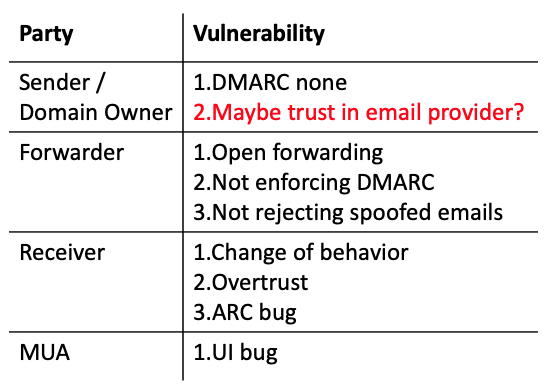
\includegraphics[width=\columnwidth]{graphs/summary_indi_vulnerabilities.png}}
% \centering
% \caption{Summary of Vulnerabilities Identified}
% \label{fig:summary_indi_vulnerabilities}
% \end{figure}

% Please add the following required packages to your document preamble:
% \usepackage{multirow}



% \subsection{Implementation Errors}
% \label{subsec:implementation_errors}
% Finally, in addition to vulnerabilities
% resulting from the design of forwarding and anti-spoofing mechanisms,
% during our experiments we also observed three implementation
% errors. We focus on Zoho's ARC implementation error, which directly
% introduces serious security concerns. The other two errors can be
% abused to help send spoofed email, which we detail in
% Appendix~\ref{sec:implementation_errors_additional}.


% in a subset of our attacks.
% Namely, Gmail's UI indicator bug and Zoho's ARC implementation bug.

% \subsubsection{Every email is legitimate}
% \grant{Hmmm... this subsection really strikes me as a broken implementation, and we might consider moving to Section 4.2}


% \subsubsection*{Zoho's ARC Implementation Error}
% \label{sec:arc}
% % \label{subsubsec:arc_bug}
% As discussed earlier in Section~\ref{sec:measure_forwarding_mechs_and_arc},
% many forwarding approaches break SPF, DKIM, and DMARC authentication.
% To remedy this compatibility issue, a new experimental protocol called Authenticated Received Chain (ARC)~\cite{rfc8617} was recently introduced to preserve email authentication results across multiple forwarders and allow the final recipient to authenticate legitimate email even if they fail DMARC authentication.
% Intermediary forwarders implementing ARC sign their authentication results
% (using new ARC headers) so that the receiver can verify each forwarder's authentication checks.
% If DMARC authentication fails, a receiver can examine the ARC validation chain to determine whether the forwarded email is legitimate~\cite{ARCSpeci1:online}.
% Although ARC can help resolve the compatibility issues with some forwarding implementations and anti-spoofing protocols, it does not remedy the security vulnerabilities presented earlier in this section.
% Additionally, ARC is currently an experimental standard and only
% implemented by a few providers~\cite{rfc8617, ARCSpeci1:online};
% Appendix~\ref{sec:appendix_arc_measurement}
% % and Table~\ref{tab:forwarding_mechs_in_the_wild}
% reports our measurement results about the adoption of ARC among
% the providers we evaluated.
% %\geoff{(will need to be updated if ARC is removed from the table)}
% Nonetheless, during our experiments, we identified attacks that can exploit incorrect ARC implementations to reliably spoof email.

% Among these platforms, many providers only accept ARC signatures from custom lists of ``trusted'' forwarders (Table~\ref{tab:trust_of_arc_between_providers}).
% During our analysis, we discovered that some email providers' implementation of ARC also leads to vulnerabilities, which an attacker can combine with forwarding to spoof malicious emails (\S~\ref{subsec:attack_zoho_arc}).
% Prior work has found that some mail providers, such as Zoho, incorrectly implement ARC~\cite{shen2020weak}.
% For example, when a spoofed email message is forwarded from Gmail to Zoho, Zoho incorrectly reads the ARC headers attached by Gmail. As a result, it incorrectly displays the email as passing DMARC and delivers the email without warnings.
% Echoing this prior work, we found that this vulnerability still existed at Zoho.
% We also found through our experiments that, in addition to Gmail, Zoho also evaluates and trusts ARC headers added by Fastmail (Section~\ref{sec:measure_forwarding_mechs_and_arc}).
% Moreover, by leveraging Fastmail's open forwarding, this flawed ARC implementation could be exploited to spoof email messages to any Zoho user from \emph{any} domain.\footnote{Our work not only led to a patch of this issue after disclosure to Zoho, but also resulted in Zoho adding additional security enhancements to their ARC implementation (Appendix~\ref{sec:disclosure}).  This patch is confirmed by the parallel work of Wang et al.~\cite{wang2022revisiting} that focused on email forwarding under ARC.}


%% \begin{figure}[t]
%%   \centering
%%   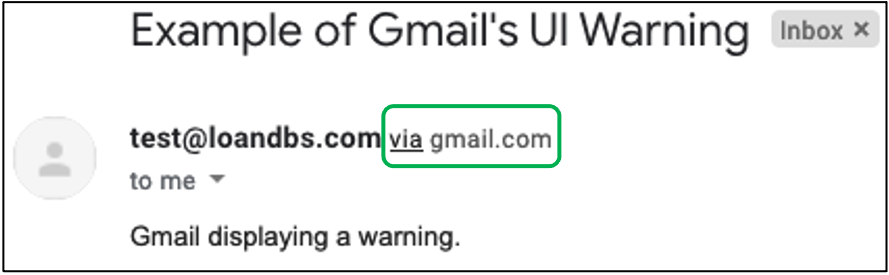
\includegraphics[width=\columnwidth]{graphs/ss_ui_warning_normal.png}
%%   \caption{Gmail's usual UI warning for forwarded mail.}
%%   \vspace*{-0.1in}
%%   \label{fig:gmail_ui_normal}
%% \end{figure}

% However, any such trust implicitly
% assumes that those trusted forwarders have good security practices.
% Unfortunately, as we detail later, this is not always the case, which
% creates additional opportunities for adversaries
% (Section~\ref{subsec:attack_zoho_arc}).
